\bichapter{改性硫化型纳米零价铁的稳定性研究}{Study on stabilization
of coated sulfur-modified NZVI}


\bisection{pH对不同包覆比的S-NZVI稳定性的影响}{Effect of pH on the stability of S-NZVI with different coating ratios}

如\cref{fig3}所示,未包覆的S-NZVI在酸性条件下时$\zeta$电位为正,碱性条件下为负,等电点在pH=7.0附近,此时颗粒表面静电力变小,排斥力减弱。由于通常地下水的pH范围在6.5到8.5之间\cite{dixiashuibiaozhun},因此该环境下未包覆的S-NZVI胶体团聚速率快,更易脱稳沉降,与相关研究结果相符。为模拟地下水环境,调节pH=8,因此本研究中的硫化纳米铁表面带负电。

\begin{figure}[h]
    \centering
    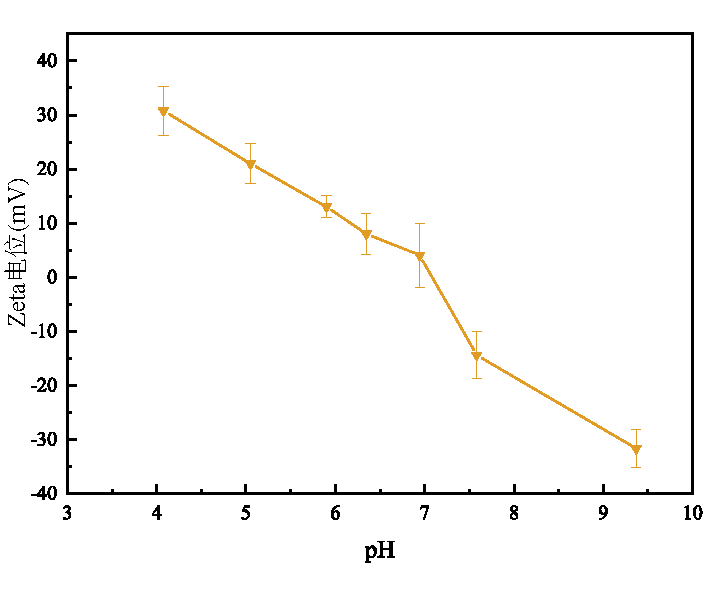
\includegraphics[width=12cm]{figs/fig3.pdf}
    \caption{不同pH裸S-NZVI的$\zeta$电位}{Zeta potential of bare S-NZVI as a function of pH}\label{fig3}
\end{figure}

\bisection{不同包覆比下S-NZVI的稳定性}{Stability of S-NZVI at different coating ratios}

纳米颗粒在水中同时受到扩散和重力沉降作用,如果纳米粒子的扩散克服了沉降作用,那么纳米粒子可以保持很长时间的稳定。其中重力作用与粒子半径的平方成正比,扩散作用与粒子尺寸成反比,当纳米粒子聚集成微米大小的团簇时,由于扩散作用小于沉降作用,团聚体会沉降到容器的底部。所以沉降速率是表征S-NZVI胶体稳定性的良好指标。

\begin{figure}[h]
    \centering
    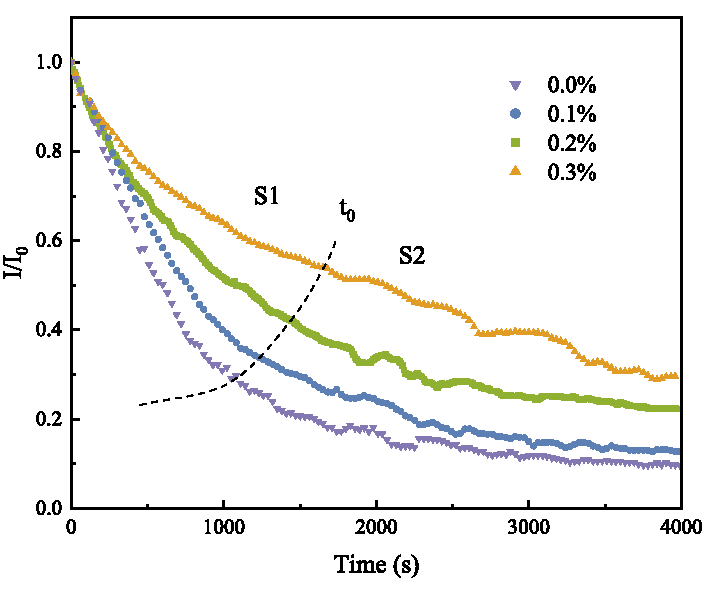
\includegraphics[width=12cm]{figs/fig1.pdf}
    \caption{不同包覆比和裸S-NZVI的沉降曲线}{Sedimentation curves of bare and modified S-NZVI}\label{fig01}
\end{figure}

如\cref{fig01}所示,未包覆的S-NZVI的沉降可分为两个阶段:在S1阶段,样品中存在大量超过临界尺寸的颗粒,因此快速沉降。在$t_0$时刻,多数大颗粒沉降完成,沉降速率降低,样品进入S2缓慢沉降阶段,逐渐趋于稳定。

海藻酸钠包覆S-NZVI的沉降模式与未包覆材料相同,均由S1、S2两个阶段组成,但由于聚电解质层的存在,包覆硫化钠米铁的沉降速率与海藻酸钠浓度负相关。海藻酸钠浓度越大,S1阶段的沉降速率越小,S2阶段保持悬浮的颗粒数量越多,体系的稳定性越好。

\bisection{离子强度对SA-S-NZVI稳定性的影响}{Effect of ionic strength on the stability of SA-S-NZVI}

金属氧化物纳米颗粒在水溶液中的稳定性在很大程度上取决于离子强度。为了研究离子强度对SA-S-NZVI在溶液中的稳定性(pH=$8\pm 0.1$),制备不同包覆比(0、0.1、0.2、0.3wt\%)的SA-S-NZVI,采用NaCl调节离子强度(0.00$\sim$100 mM NaCl)。颗粒之间的附着效率由\cref{alpha_ppexp}计算,其中$k_{\mathrm{fast}}$取扩散限制团聚阶段下$k$的平均值。

\begin{figure}[h]
    \centering
   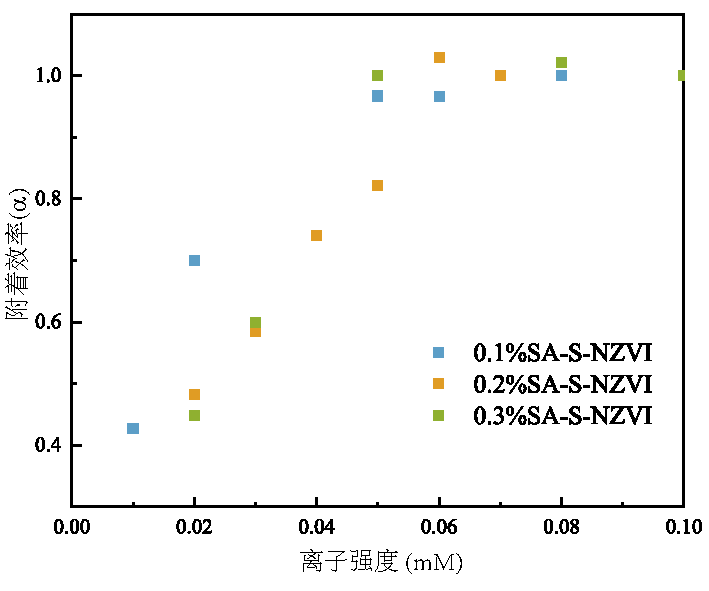
\includegraphics[width=12cm]{figs/Graph1.png}
    \bicaption{不同离子强度下包覆型S-NZVI的附着效率}{Influence of iron strength on aggreation behaviors of modified S-NZVI}\label{fig4}
\end{figure}

实验结果如\cref{fig4}所示,不同包覆比的SA-S-NZVI与裸S-NZVI随着离子强度的增加,在低浓度NaCl下,NaCl浓度的增加将提高电荷屏蔽的程度,从而提高团聚速率,这反映在附着效率的提高上。该过程中,附着效率与NaCl的投加量正相关,这种团聚过程称为反应限制团聚$(\alpha<1)$。在高NaCl浓度下,SA-NZVI的电荷被完全屏蔽,势垒消失,该过程中颗粒发生扩散限制团聚$(\alpha=1)$,团聚速率达到最大值,且与NaCl投加量无关。NaCl对不同包覆比S-NZVI的临界浓度均在0.05\textasciitilde0.06 mM附近。

\bisection{聚电解质包覆层的特性}{Characteristics of the polyelectrolyte
layers}

颗粒间空间斥力的大小和作用范围与表面吸附的聚合物浓度和包覆层厚度有关。不同包覆比的S-NZVI的电泳迁移率随离子强度的变化如\cref{fig5}所示,其中曲线由测量的平均电泳迁移率\cref{psidon,psi0,ue}拟合得到,各参数见\cref{tb1}。

由于包覆层的存在,SA-S-NZVI周围的扩散层被压缩,其电泳迁移率随离子强度的变化较未包覆S-NZVI小。随着离子强度不断提高,未包覆S-NZVI的电泳迁移率逐渐趋于零,而不同包覆比的SA-S-NZVI(0.1\%wt,0.2\%wt,0.3\%wt)受包覆层特性影响分别趋于-2.8,-2.2和-2.3 $\mathrm{\mu m\, s^{-1}\, cm\,V^{-1}} $。

由于软粒子对滑移面位置不敏感\cite{1992Electrophoretic},Smoluchoski公式以硬粒子为基础并不适用于包覆型S-NZVI。根据Ohshima的软粒子理论计算的包覆型S-NZVI的表面电荷$\psi_0$远小于由Smoluchoski公式计算的$\zeta$电位。因此,软粒子并不适用于传统DLVO理论的双电层公式计算静电斥力。

\begin{figure}[h]
    \centering
    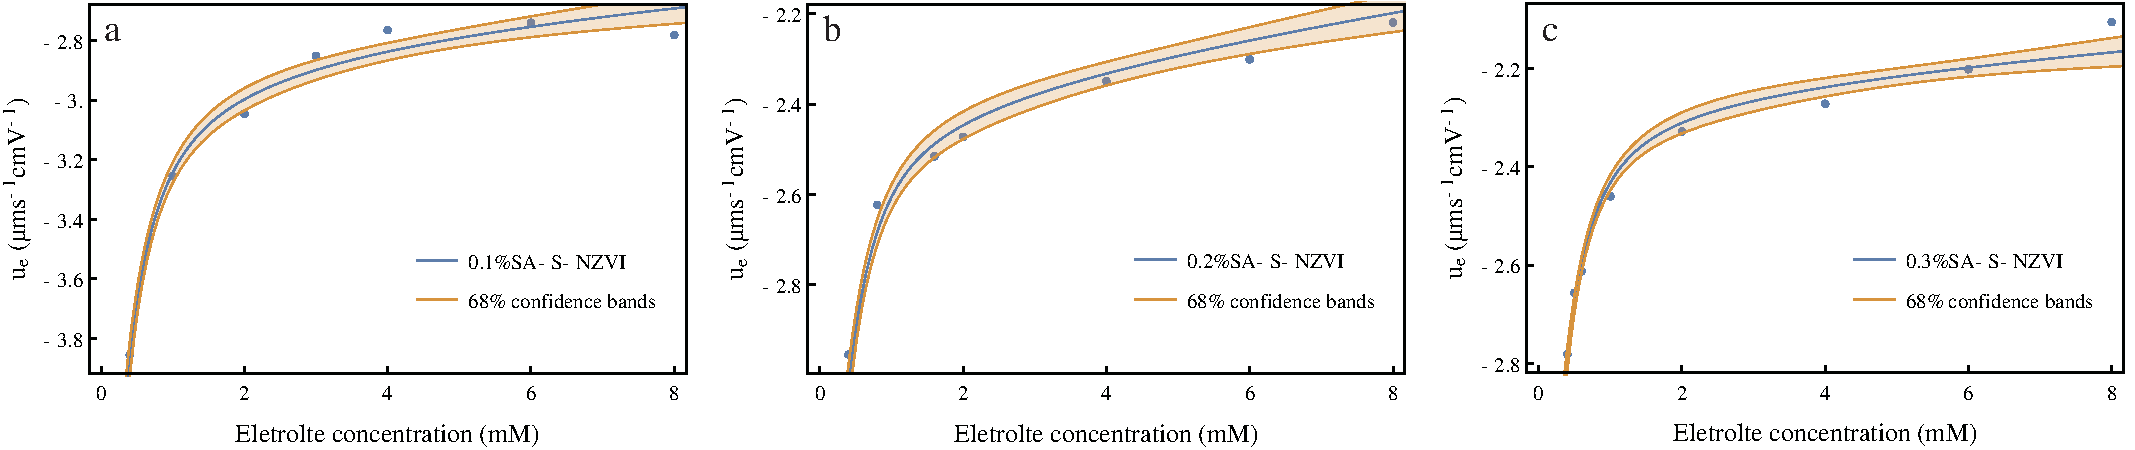
\includegraphics[width=12cm]{figs/fig5.pdf}
    \bicaption{不同NaCl浓度下包覆型S-NZVI的电泳迁移率}{Electiophoretic mobility of the sodium alginate coated S-NZVI as a function of NaCl (mM)}
    \label{fig5}
\end{figure}

\begin{table}
    \centering
    \bicaption{利用Ohshima软粒子理论计算pH值为8.0$\pm $0.1时吸附聚电解质层的特性  }{Characteristics of the adsorbed polyelectrolyte layers at pH 8.0$\pm $0.1 as estimated by Ohshima’s soft particle analysis}\label{tb1}
    \begin{tabular}{@{}ccccc@{}}
        \toprule
         样品类型 & $ZN$/$\mathrm{N_A}$& $d$ & $1/\lambda$ &$\phi_p$\\
           &$(\mathrm{mol/m^3})$&(nm)&(nm)& $(10^{-3})$ \\
        \midrule
        0.1\%SA & 3.28$\pm$1.08 & 7.97$\pm$4.11 & 6.63$\pm$0.58 & 113\\
        0.2\%SA & 1.47$\pm$1.25 & 10.94$\pm$4.68 & 8.51$\pm$1.06 & 80\\
        0.3\%SA & 1.50$\pm$1.39 & 16.62$\pm$4.58 & 9.57$\pm$1.97 & 54\\
        \bottomrule
    \end{tabular}
\end{table}


包覆层中聚电解质的体积分数是影响颗粒稳定性的重要因素。根据计算的颗粒平均包覆层厚度和吸附浓度估算吸附到NZVI表面聚电解质的体积分数:

\begin{align}
    \phi_p=& \frac{\Gamma\cdot 4\pi a^2}{\rho_p\cdot \frac{4}{3}\pi [(d+a)^3-a^3]}  \\
    =&\frac{3\cdot\Gamma a^2}{\rho_p[(d+a)^3-a^3]} \nonumber
\end{align}

其中,$\rho_p$是聚电解质密度;$d$为包覆层厚度;$a$为颗粒粒径;$\Gamma$为S-NZVI表面聚电解质的吸附浓度,制备样品吸附后通过差量法利用总有机碳分析仪测量TOC计算。

\bisection{本章小结}{Result}